\documentclass[11pt,a4paper]{article}

\usepackage[slovene]{babel}
\usepackage{color}
\usepackage{graphicx}

\begin{document}

\title{Nihalo v viskoznem mediju}
\author{\v Ziga Pata\v cko Koderman}
\date{\today}

\maketitle

\section{Fizikalno ozadje}

Gibanje nihala, potopljenega v viskoznem mediju, opi\v semo s slede\v co diferencialno ena\v cbo:

$$
\frac{d^2\phi}{dt^2} + \frac{6 \pi \eta r}{m} \frac{d\phi}{dt} + \frac{g}{l}sin(\phi) = 0
$$

Uvedemo brezdimenzijski \v cas $\tau = t\sqrt{\frac{g}{l}}$ ter brezdimenzijski koeficient du\v senja $\beta = \frac{6 \pi \eta r}{m} \sqrt{\frac{l}{g}}$:

$$
\frac{d\phi}{dt} = \frac{d\phi}{d\eta} \frac{d\eta}{dt} = \frac{d\phi}{d\tau} \sqrt{\frac{g}{l}}
$$

ter prvotno ena\v cbo preoblikujemo v brezdimenzijsko:

$$
\frac{d^2\phi}{d\tau ^2} + \beta \frac{d\phi}{d\tau} + sin(\phi) = 0
$$

Ena\v cbo dalje re\v sujemo numeri\v cno.

\section{Rezultati}

Za koeficiente $\beta \in \{ 0.02, 0.05, 0.1, 0.2 \} $ izri\v semo grafa odmika in energije v odvisnosti od brezdimenzijskega \v casa $\tau$. Energijo definiramo kot:

$$
E = \frac{1}{2}(\frac{d\phi}{d\tau})^2 + \frac{1}{2}(1 - cos(\phi))
$$

%\vspace{1cm}

\begin{figure}
  \begin{center}
  	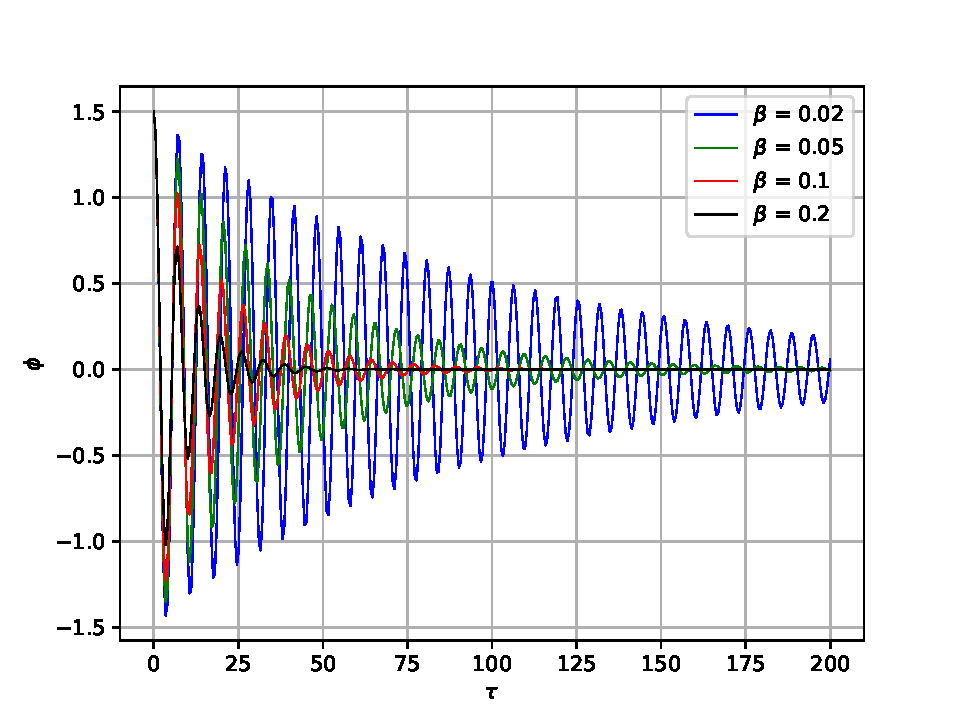
\includegraphics[width=12cm]{graf1.pdf}
    \caption{Graf $\phi$ v odvisnosti od $\tau$}
  \end{center}
\end{figure}

\begin{figure}
  \begin{center}
  	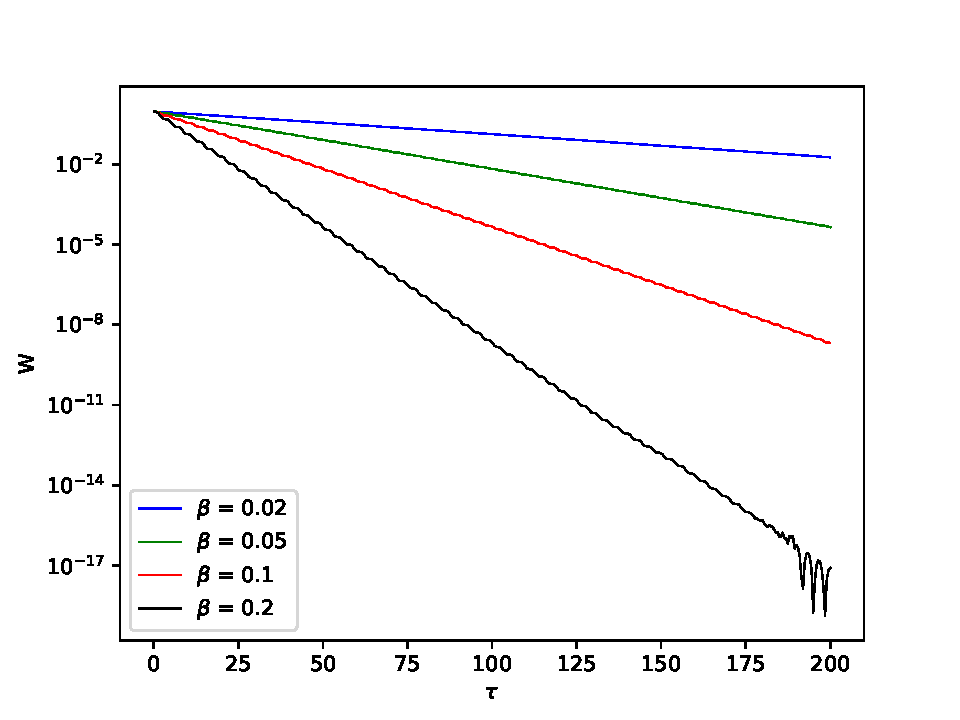
\includegraphics[width=12cm]{graf2.pdf}
    \caption{Graf energije v odvisnosti od $\tau$ v logaritmski skali}
  \end{center}
\end{figure}

\vspace{2cm}

\section{Interpretacija}
Energija du\v senega nihala pada v logaritemski skali linearno s koeficientom $\beta$. Predvidevamo torej, da za energijo na\v sega nihala velja:
$$
E = E_0 e^{-\beta\tau}
$$

Graf energije v odvisnosti od $\tau$ pa ni raven - niha okoli premice. Za to \v zal nisem uspel najti nobene fizikalno smiselne razlage, zato to pripisujem numeri\v cni napaki ra\v cunalnika (pri zelo majhnih \v stevilih je vse ve\v cja, posebej pa se to vidi pri $\beta = 0.2$ in \v casih $ \tau > 180$).
\end{document}
